\documentclass[10pt,a4paper]{article}
\usepackage[T1]{fontenc}
\usepackage{lmodern}
\usepackage[margin=1.7cm]{geometry}
\usepackage{amsmath,amssymb}
\usepackage{booktabs,array,tabularx}
\usepackage{enumitem}
\usepackage[dvipsnames]{xcolor}
\usepackage{tikz}
\usetikzlibrary{arrows.meta,positioning,shapes.geometric}
\usepackage[most]{tcolorbox}
\usepackage{fancyhdr}
\usepackage[colorlinks=true,linkcolor=NavyBlue,urlcolor=NavyBlue]{hyperref}

\setlist{nosep,leftmargin=*}
\setlength{\parindent}{0pt}
\setlength{\parskip}{3pt}

\pagestyle{fancy}
\fancyhf{}
\lhead{\small BACSE202 -- Module 4 (Slides 1--90)}
\rhead{\small Transaction Processing \& Schedules}
\cfoot{\thepage}

\newtcolorbox{keybox}[1][]{colback=NavyBlue!5,colframe=NavyBlue!70,fonttitle=\bfseries,title=#1,boxsep=2pt,left=4pt,right=4pt,top=2pt,bottom=2pt}
\newtcolorbox{exbox}[1][]{colback=ForestGreen!5,colframe=ForestGreen!70,fonttitle=\bfseries,title=#1,boxsep=2pt,left=4pt,right=4pt,top=2pt,bottom=2pt}
\newtcolorbox{warnbox}[1][]{colback=BrickRed!5,colframe=BrickRed!70,fonttitle=\bfseries,title=#1,boxsep=2pt,left=4pt,right=4pt,top=2pt,bottom=2pt}

\newcommand{\op}[1]{\texttt{#1}}
\newcommand{\ri}[2]{r_{#1}(#2)}
\newcommand{\wi}[2]{w_{#1}(#2)}

\begin{document}

\begin{center}
{\LARGE\bfseries BACSE202 -- Database Systems}\\[3pt]
{\Large Module 4: Transaction Processing -- Quick Exam Notes}\\[3pt]
{\small Covers slides 1--90 of \texttt{BACSE202-DBS-Module-4.ppt} (Elmasri \& Navathe Ch.~21; Silberschatz Ch.~14)}
\end{center}

\tableofcontents
\vspace{4pt}\hrule

%=====================================================================
\section{Transactions -- Basics (Slides 3--14)}

\begin{keybox}[Definition]
A \textbf{transaction} is a \emph{unit of program execution} that accesses and possibly updates data items -- a \textbf{logical unit of database processing}.
\end{keybox}

\begin{itemize}
  \item \textbf{Main operations:} \emph{read} (retrieval, e.g.\ SQL \op{SELECT}) and \emph{write} (modify, e.g.\ \op{INSERT}, \op{UPDATE}, \op{DELETE}).
  \item Example: transfer \$100 from a checking account to a savings account.
  \item A transaction is either \textbf{stand-alone} (SQL typed interactively) or \textbf{embedded} in a program (most transactions).
  \item \textbf{Transaction processing systems}: large multi-user systems running thousands of concurrent transactions per minute (banking, airline reservations).
\end{itemize}

\subsection*{Two modes of concurrency (Fig.~21.1)}
\begin{itemize}
  \item \textbf{Interleaved processing:} one CPU; operations of transactions A and B are interleaved over time ($t_1$--$t_2$).
  \item \textbf{Parallel processing:} multiple CPUs; C runs on CPU$_1$ while D runs on CPU$_2$ ($t_3$--$t_4$).
  \item Basic transaction theory assumes \textbf{interleaved} concurrency.
\end{itemize}

\subsection*{Basic operations on a data item $X$}
\begin{tabularx}{\linewidth}{@{}l X@{}}
\toprule
\op{read\_item(X)} & 1.~Find the address of the disk block containing $X$. 2.~Copy that block into a main-memory buffer (if not already there). 3.~Copy $X$ from the buffer into program variable $X$.\\
\op{write\_item(X)} & 1.~Find the block address. 2.~Copy the block into a buffer (if not there). 3.~Copy program variable $X$ into its place in the buffer. 4.~Store the updated block back to disk -- \emph{immediately or later}.\\
\bottomrule
\end{tabularx}

\subsection*{Operations tracked by the Recovery Manager}
\begin{enumerate}
  \item \op{begin\_transaction} -- start of execution.
  \item \op{read} / \op{write} -- operations on items.
  \item \op{end\_transaction} -- reads/writes are over; now check whether changes can be \emph{committed} or the transaction must be \emph{aborted} (e.g.\ violates concurrency control).
  \item \op{commit\_transaction} -- successful end; changes are permanent.
  \item \op{rollback} / \op{abort} -- unsuccessful end; changes must be undone.
\end{enumerate}

\subsection*{Notation (Fig.~21.2)}
\begin{minipage}{0.48\linewidth}
\begin{tabular}{@{}ll@{}}
\toprule
$T_1$ & $T_2$\\\midrule
\op{read\_item(X);} & \op{read\_item(X);}\\
$X := X - N$; & $X := X + M$;\\
\op{write\_item(X);} & \op{write\_item(X);}\\
\op{read\_item(Y);} & \\
$Y := Y + N$; & \\
\op{write\_item(Y);} & \\
\bottomrule
\end{tabular}
\end{minipage}\hfill
\begin{minipage}{0.48\linewidth}
Shorthand:\\
$T_1: b_1; \ri1X; \wi1X; \ri1Y; \wi1Y; e_1;$\\
$T_2: b_2; \ri2X; \wi2X; e_2;$\\[2pt]
$b_i,e_i$ = begin/end; $i$ = transaction id. Later also $c_i$ (commit), $a_i$ (abort).
\end{minipage}

%=====================================================================
\section{Why Concurrency Control is Needed (Slides 15--19)}

\begin{tabularx}{\linewidth}{@{}>{\raggedright\arraybackslash}p{3.2cm} X@{}}
\toprule
\textbf{Problem} & \textbf{What happens}\\\midrule
\textbf{Lost Update} (Fig.~21.3a) & Two transactions read the \emph{same original} value of $X$ and both update it; one update overwrites the other.\\
\textbf{Temporary Update / Dirty Read} (Fig.~21.3b) & $T_1$ writes $X$, $T_2$ reads that $X$, then $T_1$ \emph{fails} and $X$ is rolled back -- $T_2$ has used a value that ``never existed''.\\
\textbf{Incorrect Summary} (Fig.~21.3c) & An aggregate (e.g.\ sum of balances) reads some values \emph{before} and others \emph{after} another transaction's update.\\
\textbf{Unrepeatable Read} & $T_1$ reads $X$ twice and gets different values because $T_2$ changed $X$ in between (e.g.\ seats on a flight).\\
\bottomrule
\end{tabularx}

\begin{exbox}[Interleavings from Fig.~21.3]
\small
\begin{tabular}{@{}p{0.2\linewidth}|p{0.2\linewidth}||p{0.2\linewidth}|p{0.2\linewidth}@{}}
\multicolumn{2}{@{}l||}{\textbf{(a) Lost update}} & \multicolumn{2}{l@{}}{\textbf{(b) Temporary update / dirty read}}\\
$T_1$ & $T_2$ & $T_1$ & $T_2$\\\hline
$r(X)$; $X{:=}X{-}N$ & & $r(X)$; $X{:=}X{-}N$ & \\
 & $r(X)$; $X{:=}X{+}M$ & $w(X)$ & \\
$w(X)$; $r(Y)$ & & & $r(X)$; $X{:=}X{+}M$\\
 & $w(X)$ \textcolor{BrickRed}{$\leftarrow$ lost} & & $w(X)$\\
$Y{:=}Y{+}N$; $w(Y)$ & & $r(Y)$ \textcolor{BrickRed}{fails} & \\
\end{tabular}

\vspace{2pt}
(a) $T_1$'s write of $X$ is overwritten by $T_2$, which used the old value. \quad
(b) $T_1$ fails and must restore the old $X$, but $T_2$ already read the \emph{temporary} value.

\vspace{4pt}
\begin{tabular}{@{}p{0.3\linewidth}|p{0.3\linewidth}@{}}
\multicolumn{2}{@{}l}{\textbf{(c) Incorrect summary}}\\
$T_1$ & $T_3$\\\hline
 & $sum{:=}0$; $r(A)$; $sum{:=}sum{+}A$; \dots\\
$r(X)$; $X{:=}X{-}N$; $w(X)$ & \\
 & $r(X)$; $sum{:=}sum{+}X$\\
 & $r(Y)$; $sum{:=}sum{+}Y$\\
$r(Y)$; $Y{:=}Y{+}N$; $w(Y)$ & \\
\end{tabular}

\vspace{2pt}
(c) $T_3$ reads $X$ \emph{after} $N$ is subtracted but $Y$ \emph{before} $N$ is added, so the sum is off by $N$.
\end{exbox}

%=====================================================================
\section{Why Recovery is Needed (Slides 20--23)}

\textbf{Causes of transaction failure:}
\begin{enumerate}
  \item \textbf{Computer failure (system crash)} -- hardware/software error; main memory contents may be lost.
  \item \textbf{Transaction or system error} -- integer overflow, division by zero, bad parameters, logical error, user interrupt.
  \item \textbf{Local errors / exception conditions} -- e.g.\ data not found, insufficient balance $\Rightarrow$ programmed abort.
  \item \textbf{Concurrency control enforcement} -- CC aborts the transaction (violates serializability or deadlock); restarted later.
  \item \textbf{Disk failure} -- blocks lost due to read/write malfunction or head crash.
  \item \textbf{Physical problems \& catastrophes} -- power/AC failure, fire, theft, sabotage, overwriting disks, wrong tape mounted.
\end{enumerate}
Failures 1--4 are common; 5--6 are more severe (need backup/archive).

\textbf{System operations during recovery:}
\begin{itemize}
  \item \op{undo(X)} -- like rollback, but for a \emph{single write} operation.
  \item \op{redo(X)} -- re-apply a write of a \emph{committed} transaction to ensure it is permanent on disk.
\end{itemize}

%=====================================================================
\section{ACID Properties (Slides 24--31)}

Running example -- transfer \$50 from $A$ to $B$:
\[
\text{1. } read(A)\quad \text{2. } A := A-50\quad \text{3. } write(A)\quad \text{4. } read(B)\quad \text{5. } B := B+50\quad \text{6. } write(B)
\]
Two main issues: \textbf{failures} (hardware, crashes) and \textbf{concurrent execution}.

\begin{tabularx}{\linewidth}{@{}p{2.3cm} X X@{}}
\toprule
\textbf{Property} & \textbf{Meaning} & \textbf{In the \$50 transfer}\\\midrule
\textbf{Atomicity} & All operations are reflected in the DB, or none. & If failure after step 3 but before step 6, \$50 is ``lost''; partial updates must not be reflected.\\
\textbf{Consistency} & A transaction run in isolation takes the DB from one consistent state to another. & $A+B$ is unchanged. Includes explicit constraints (PK, FK) and implicit ones (e.g.\ total balances $-$ loans $=$ cash-in-hand). DB may be temporarily inconsistent during execution. DBMS guarantees consistency only if the transaction logic is correct.\\
\textbf{Isolation} & Concurrent execution must be equivalent to some serial execution; intermediate results not visible. For every $T_i,T_j$: to $T_i$ it appears $T_j$ finished before $T_i$ started or started after $T_i$ finished. & If $T_2$ runs \texttt{read(A), read(B), print(A+B)} between steps 3 and 6, it sees $A+B$ \emph{less} than it should be. Trivial solution: run serially -- but concurrency has big benefits.\\
\textbf{Durability} & Once committed, changes persist despite failures. & After the user is told the transfer is done, the updates must survive any crash.\\
\bottomrule
\end{tabularx}

\begin{keybox}[Who ensures what]
Atomicity \& Durability $\to$ \textbf{recovery manager}; Isolation $\to$ \textbf{concurrency-control} subsystem; Consistency $\to$ \textbf{programmer} + integrity constraints.
\end{keybox}

%=====================================================================
\section{Transaction States (Slides 32--35)}

\begin{minipage}{0.52\linewidth}
\begin{itemize}
  \item \textbf{Active} -- initial state while executing (reads/writes).
  \item \textbf{Partially committed} -- after the final statement executes.
  \item \textbf{Failed} -- normal execution cannot proceed.
  \item \textbf{Aborted} -- rolled back, DB restored to its prior state. Then either \emph{restart} (only if no internal logical error) or \emph{kill}.
  \item \textbf{Committed} -- after successful completion.
  \item \textbf{Terminated} (Elmasri Fig.~21.4) -- leaves the system after commit or failure.
\end{itemize}
\end{minipage}\hfill
\begin{minipage}{0.46\linewidth}
\centering
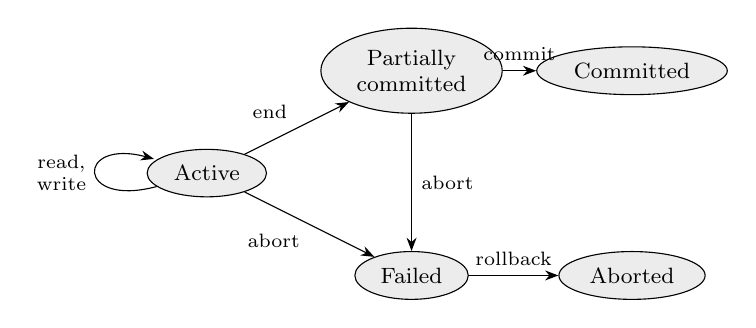
\begin{tikzpicture}[>=Stealth,st/.style={draw,ellipse,fill=gray!15,font=\footnotesize,minimum height=6mm,align=center}]
\node[st] (a) at (0,0) {Active};
\node[st] (p) at (2.6,1.3) {Partially\\committed};
\node[st] (f) at (2.6,-1.3) {Failed};
\node[st] (c) at (5.4,1.3) {Committed};
\node[st] (ab) at (5.4,-1.3) {Aborted};
\draw[->] (a) -- node[above left,font=\scriptsize]{end} (p);
\draw[->] (a) -- node[below left,font=\scriptsize]{abort} (f);
\draw[->] (p) -- node[right,font=\scriptsize]{abort} (f);
\draw[->] (p) -- node[above,font=\scriptsize]{commit} (c);
\draw[->] (f) -- node[above,font=\scriptsize]{rollback} (ab);
\draw[->] (a) edge[loop left] node[left,font=\scriptsize,align=center]{read,\\write} (a);
\end{tikzpicture}
\end{minipage}

\subsection*{Implementing Atomicity \& Durability -- Shadow-database scheme}
\begin{itemize}
  \item The \textbf{recovery-management component} implements atomicity and durability.
  \item All updates are made on a \textbf{shadow copy} of the database.
  \item \op{db\_pointer} is switched to the updated copy only after the transaction reaches \emph{partial commit} and all updated pages are \emph{flushed to disk}. The old copy is then deleted.
  \item Failure before the switch $\Rightarrow$ old copy still valid (atomicity). After the switch $\Rightarrow$ new copy permanent (durability).
\end{itemize}

%=====================================================================
\section{Concurrent Executions and Schedules (Slides 36--46)}

\textbf{Why allow concurrency?}
\begin{itemize}
  \item \textbf{Better CPU and disk utilisation} $\Rightarrow$ higher throughput (one transaction uses the CPU while another does I/O).
  \item \textbf{Reduced average response time} -- short transactions need not wait behind long ones.
\end{itemize}
\textbf{Concurrency-control schemes} = mechanisms to achieve isolation, i.e.\ control the interaction among concurrent transactions so they don't destroy consistency.

\begin{keybox}[Schedule]
A \textbf{schedule (history)} is a sequence of instructions giving the chronological order in which instructions of concurrent transactions execute. It must contain \emph{all} instructions of those transactions and \emph{preserve the order within each transaction}. A completed transaction ends with \textbf{commit}; a failed one with \textbf{abort}.
\end{keybox}

\textbf{Formal definition:} A schedule $S$ of $T_1,\dots,T_n$ is an ordering of all their operations such that, for each $T_i$, the operations of $T_i$ appear in $S$ in the same order as in $T_i$ (other transactions' operations may be interleaved).

\textbf{Number of possible schedules} (each $T_i$ has $m_i$ operations):
\[
\frac{(m_1+m_2+\dots+m_n)!}{m_1!\; m_2!\; \cdots\; m_n!}
\]
E.g.\ $T_1$ with 4 ops and $T_2$ with 2 ops: $\dfrac{6!}{4!\,2!}=15$ schedules.

\subsection*{Silberschatz schedules: $T_1$ transfers \$50 $A\to B$; $T_2$ transfers 10\% of $A$ to $B$ (start $A=100$, $B=200$)}

\begin{minipage}[t]{0.48\linewidth}
\small
$T_1$: \texttt{read(A); A:=A-50; write(A); read(B); B:=B+50; write(B)}\\
$T_2$: \texttt{read(A); temp:=A*0.1; A:=A-temp; write(A); read(B); B:=B+temp; write(B)}
\end{minipage}\hfill
\begin{minipage}[t]{0.5\linewidth}
\small
\begin{tabular}{@{}lllc@{}}
\toprule
\textbf{Schedule} & \textbf{Order} & \textbf{Final $A,B$} & $A+B$\\\midrule
1 (serial) & $T_1$ then $T_2$ & 45, 255 & 300 \checkmark\\
2 (serial) & $T_2$ then $T_1$ & 40, 260 & 300 \checkmark\\
3 (concurrent) & equivalent to 1 & 45, 255 & 300 \checkmark\\
4 (concurrent) & \emph{not} serializable & \textbf{50, 210} & \textbf{260} $\times$\\
\bottomrule
\end{tabular}
\end{minipage}

\vspace{3pt}
\begin{exbox}[Schedule 3 vs.\ Schedule 4 (step by step)]
\small
\begin{minipage}[t]{0.49\linewidth}
\textbf{Schedule 3} (non-serial, but equivalent to 1)\\
$T_1$: read(A)=100, $A$=50, write(A) $\to A{=}50$\\
$T_2$: read(A)=50, temp=5, $A$=45, write(A) $\to A{=}45$\\
$T_1$: read(B)=200, $B$=250, write(B) $\to B{=}250$\\
$T_2$: read(B)=250, $B$=255, write(B) $\to B{=}255$\\
Final $A+B = 45+255 = 300$ \checkmark
\end{minipage}\hfill
\begin{minipage}[t]{0.49\linewidth}
\textbf{Schedule 4} (does NOT preserve $A+B$)\\
$T_1$: read(A)=100, $A$=50 (not yet written)\\
$T_2$: read(A)=100, temp=10, $A$=90, write(A) $\to A{=}90$, read(B)=200\\
$T_1$: write(A) $\to A{=}50$ (overwrites 90!), read(B)=200, $B$=250, write(B)\\
$T_2$: $B$=200+10=210, write(B) $\to B{=}210$ (overwrites 250!)\\
Final $A+B = 50+210 = 260$ $\times$ \;(\$40 vanished -- lost updates)
\end{minipage}
\end{exbox}
\begin{warnbox}[Slide 41 correction]
The slide's value table for Schedule 4 shows $A=90$, $B=250/260$, $A+B=340/350$. Tracing the operations gives \textbf{$A=50$, $B=210$, $A+B=260$} (Silberschatz: with $A=1000,B=2000$ the result is $950+2100$). Either way the sum is \emph{not} preserved.
\end{warnbox}

\subsection*{Elmasri Fig.~21.5 -- Schedules A--D of $T_1,T_2$ (compact notation)}
\begin{tabular}{@{}ll@{}}
\textbf{A} (serial $T_1T_2$) & $\ri1X;\ \wi1X;\ \ri1Y;\ \wi1Y;\ \ri2X;\ \wi2X$\\
\textbf{B} (serial $T_2T_1$) & $\ri2X;\ \wi2X;\ \ri1X;\ \wi1X;\ \ri1Y;\ \wi1Y$\\
\textbf{C} (non-serial) & $\ri1X;\ \ri2X;\ \wi1X;\ \ri1Y;\ \wi2X;\ \wi1Y$ \quad (lost update!)\\
\textbf{D} (non-serial) & $\ri1X;\ \wi1X;\ \ri2X;\ \wi2X;\ \ri1Y;\ \wi1Y$\\
\end{tabular}

Some schedules are easy to recover from, some not (\textbf{recoverability}); some give correct results, some not (\textbf{serializability}).

%=====================================================================
\section{Schedules Based on Recoverability (Slides 47--55)}

\begin{keybox}[Definitions]
\begin{itemize}
  \item \textbf{Recoverable:} no committed transaction ever needs to be rolled back. Formally: \emph{no $T$ commits until every $T'$ that wrote an item $T$ read has committed.}
  \item \textbf{Non-recoverable:} a committed transaction may have to be rolled back -- violates \emph{durability}; must not be allowed.
  \item \textbf{Cascading rollback:} an uncommitted $T_2$ that read from a failed $T_1$ must also be rolled back.
  \item \textbf{Cascadeless (ACA):} $T_2$ cannot \emph{read} $X$ until the $T_1$ that last wrote $X$ has committed/aborted.
  \item \textbf{Strict:} $T_2$ can neither \emph{read nor write} $X$ until the $T_1$ that last wrote $X$ has committed/aborted.
  \item \textbf{Blind write:} $w_2(X)$ not preceded by $r_2(X)$.
\end{itemize}
\end{keybox}

\begin{center}
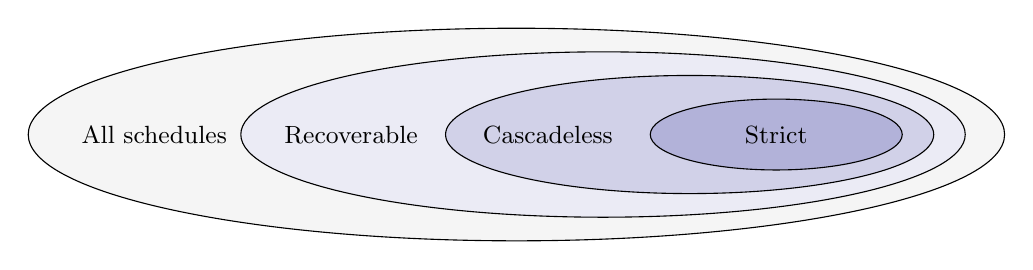
\begin{tikzpicture}
\draw[fill=gray!8] (0,0) ellipse (6.2 and 1.35); \node at (-4.6,0) {\small All schedules};
\draw[fill=NavyBlue!8] (1.1,0) ellipse (4.6 and 1.05); \node at (-2.1,0) {\small Recoverable};
\draw[fill=NavyBlue!18] (2.2,0) ellipse (3.1 and 0.75); \node at (0.4,0) {\small Cascadeless};
\draw[fill=NavyBlue!30] (3.3,0) ellipse (1.6 and 0.45); \node at (3.3,0) {\small Strict};
\end{tikzpicture}\\
{\small Strict $\subseteq$ Cascadeless $\subseteq$ Recoverable $\subseteq$ All. \; If blind writes are \emph{not} allowed: Cascadeless $=$ Strict.}
\end{center}

\begin{exbox}[Slide examples]
\small
\begin{tabularx}{\linewidth}{@{}l X X@{}}
\toprule
\textbf{Schedule} & \textbf{Operations} & \textbf{Verdict}\\\midrule
A & $\ri1X$; $\wi1X$; $\ri2X$; $\wi2X$; $c_2$; $\ri1Y$; $\wi1Y$; $c_1$ (or $a_1$) & \textbf{Non-recoverable}: $T_2$ read $X$ from $T_1$ and commits first. If $T_1$ aborts, committed $T_2$ is wrong.\\
B & $\ri1X$; $\wi1X$; $\ri2X$; $\wi2X$; $\ri1Y$; $\wi1Y$; $c_1$ (or $a_1$)$; $\dots & \textbf{Recoverable} ($c_2$ delayed until after $c_1$); if $T_1$ aborts, $T_2$ must abort $\Rightarrow$ \emph{cascading rollback}; \textbf{not cascadeless}.\\
C & $\ri1X$; $\wi1X$; $\ri1Y$; $\wi1Y$; $c_1$; $\ri2X$; $\wi2X$; $\dots$ & \textbf{Cascadeless} and \textbf{strict} ($r_2(X)$ delayed until $T_1$ commits; no blind writes).\\
D & $\ri1X$; $\wi1X$; $\wi3X$; $\ri1Y$; $\wi1Y$; $c_1$; $\ri2X$; $\wi2X$; $\dots$ & \textbf{Cascadeless but not strict}: blind write $w_3(X)$ before $T_1$ commits.\\
E & $\ri1X$; $\wi1X$; $\ri1Y$; $\wi1Y$; $c_1$; $\wi3X$; $\ri2X$; $\wi2X$; $\dots$ & \textbf{Strict} ($w_3(X)$ delayed until after $c_1$).\\
\bottomrule
\end{tabularx}

\vspace{3pt}
Quick patterns (slide 53):\;
$w_1(X)\ r_2(X)\ c_2\ c_1$ $\to$ \textbf{non-recoverable};\;
$w_1(X)\ r_2(X)\ c_1\ c_2$ $\to$ \textbf{recoverable} (not cascadeless -- $T_2$ read uncommitted data);\;
$w_1(X)\ c_1\ r_2(X)\ c_2$ $\to$ \textbf{recoverable, cascadeless, strict}.
\end{exbox}

\begin{warnbox}[Slide 53 note]
The slide labels ``$w_1(X)\ r_2(X)\ c_1\ c_2$'' as \emph{Recoverable Cascadeless}. By the definition on slide 49 it is recoverable but \textbf{not} cascadeless, because $r_2(X)$ reads $X$ before $T_1$ commits.
\end{warnbox}

\begin{tabular}{@{}ll@{}}
\toprule
\textbf{Property} & \textbf{Condition} (if $T_i$ wrote $X$ and $T_j$ is another transaction)\\\midrule
Recoverable & $T_j$ commits only after $T_i$ commits, if $T_j$ read from $T_i$\\
Cascadeless & $T_j$ cannot \emph{read} $X$ until $T_i$ commits\\
Strict & $T_j$ cannot \emph{read or write} $X$ until $T_i$ commits\\
\bottomrule
\end{tabular}

%=====================================================================
\section{Schedules Based on Serializability (Slides 56--67)}

\begin{itemize}
  \item Each transaction on its own is correct (consistency preservation).
  \item \textbf{Serial schedule:} all operations of each transaction execute consecutively, no interleaving. Otherwise \textbf{non-serial}. Every serial schedule is \textbf{correct}.
  \item Serial schedules are \textbf{not feasible for performance}: no interleaving; long transactions make others wait; CPU idles during I/O.
  \item \textbf{Serializable schedule:} equivalent to \emph{some} serial schedule of the same $n$ transactions. There are $n!$ serial schedules.
\end{itemize}

\subsection*{Equivalence of schedules}
\begin{itemize}
  \item \textbf{Result equivalent:} same final DB state. Not reliable -- may hold ``by chance''. Fig.~21.6: $S_1$: $X := X + 10$ and $S_2$: $X := X \times 1.1$ both give 110 when $X=100$, but differ for other values.
  \item \textbf{Conflict equivalent:} the relative order of \emph{every pair of conflicting operations} is the same in both schedules (the commonly used definition).
\end{itemize}

\begin{keybox}[Conflicting operations]
Two operations conflict iff (1) they access the \textbf{same item}, (2) they belong to \textbf{different transactions}, and (3) \textbf{at least one is a write}.\\
\par\centering
\begin{tabular}{cccc}
\toprule
$T_i$ & $T_j$ & Conflict? & Type\\\midrule
R(X) & R(X) & No & --\\
R(X) & W(X) & Yes & read--write\\
W(X) & R(X) & Yes & write--read\\
W(X) & W(X) & Yes & write--write\\
\bottomrule
\end{tabular}
\end{keybox}
Swapping conflicting operations changes the outcome: $r_1(X);w_2(X)\to w_2(X);r_1(X)$ makes $T_1$ read a different value; $w_1(Y);w_2(Y)\to w_2(Y);w_1(Y)$ changes the final $Y$. Swapping reads $r_1(Z);r_2(Z)$ changes nothing.

\begin{itemize}
  \item $S$ is \textbf{(conflict) serializable} if it is conflict equivalent to some serial schedule $S'$.
  \item A serializable schedule is \textbf{correct} (same as a serial one) yet gains the \textbf{efficiency} of interleaving.
  \item Serializability is \textbf{hard to check at run time} (OS scheduler decides interleaving; transactions continuously start and end).
  \item \textbf{Practical approach:} use \textbf{concurrency-control protocols} that guarantee serializability -- in most DBMSs, \textbf{two-phase locking (2PL)}.
\end{itemize}

%=====================================================================
\section{Testing Conflict Serializability -- Precedence Graph (Slides 68--72)}

\begin{keybox}[Algorithm 21.1]
\begin{enumerate}
  \item Create a node for each transaction $T_i$ in $S$.
  \item Edge $T_i\to T_j$ if $T_j$ does \op{read\_item(X)} \emph{after} $T_i$ does \op{write\_item(X)}. \hfill (W--R)
  \item Edge $T_i\to T_j$ if $T_j$ does \op{write\_item(X)} \emph{after} $T_i$ does \op{read\_item(X)}. \hfill (R--W)
  \item Edge $T_i\to T_j$ if $T_j$ does \op{write\_item(X)} \emph{after} $T_i$ does \op{write\_item(X)}. \hfill (W--W)
  \item $S$ is conflict serializable \textbf{iff the graph has no cycle}. An equivalent serial order = a \textbf{topological sort} of the graph.
\end{enumerate}
\end{keybox}

\begin{exbox}[Fig.~21.7 -- Schedules A--D]
\small
\begin{minipage}{0.6\linewidth}
\begin{itemize}
  \item \textbf{A:} $T_1\to T_2$ (on $X$) -- serial.
  \item \textbf{B:} $T_2\to T_1$ (on $X$) -- serial.
  \item \textbf{C:} $\ri1X$ before $\wi2X$ gives $T_1\to T_2$; $\ri2X$ before $\wi1X$ gives $T_2\to T_1$ $\Rightarrow$ \textbf{cycle $\Rightarrow$ not serializable}.
  \item \textbf{D:} only $T_1\to T_2$ $\Rightarrow$ \textbf{serializable}, equivalent to A.
\end{itemize}
\end{minipage}\hfill
\begin{minipage}{0.36\linewidth}
\centering
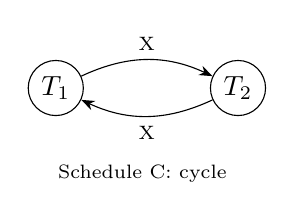
\begin{tikzpicture}[>=Stealth,n/.style={draw,circle,inner sep=1pt,minimum size=7mm}]
\node[n] (a) {$T_1$}; \node[n,right=1.6cm of a] (b) {$T_2$};
\draw[->] (a) to[bend left=25] node[above,font=\scriptsize]{X} (b);
\draw[->] (b) to[bend left=25] node[below,font=\scriptsize]{X} (a);
\node[below=0.5cm of a,xshift=1.1cm,font=\scriptsize] {Schedule C: cycle};
\end{tikzpicture}
\end{minipage}
\end{exbox}

\begin{exbox}[Fig.~21.8 -- three transactions]
\small
$T_1: r(X); w(X); r(Y); w(Y)$ \qquad $T_2: r(Z); r(Y); w(Y); r(X); w(X)$ \qquad $T_3: r(Y); r(Z); w(Y); w(Z)$

\textbf{Schedule E:} $\ri2Z;\ \ri2Y;\ \wi2Y;\ \ri3Y;\ \ri3Z;\ \ri1X;\ \wi1X;\ \wi3Y;\ \wi3Z;\ \ri2X;\ \ri1Y;\ \wi1Y;\ \wi2X$\\
Edges: $T_1\to T_2$ ($X$), $T_2\to T_1$ ($Y$), $T_2\to T_3$ ($Y,Z$), $T_3\to T_1$ ($Y$).\\
Cycles $T_1\to T_2\to T_1$ and $T_1\to T_2\to T_3\to T_1$ $\Rightarrow$ \textbf{not serializable} (no equivalent serial schedule).

\textbf{Schedule F:} $\ri3Y;\ \ri3Z;\ \ri1X;\ \wi1X;\ \wi3Y;\ \wi3Z;\ \ri2Z;\ \ri1Y;\ \wi1Y;\ \ri2Y;\ \wi2Y;\ \ri2X;\ \wi2X$\\
Edges: $T_3\to T_1$ ($Y$), $T_3\to T_2$ ($Y,Z$), $T_1\to T_2$ ($X,Y$). No cycle $\Rightarrow$ \textbf{serializable}, equivalent to $T_3\to T_1\to T_2$.

\textbf{(f)} A graph with only $T_3\to T_1$ and $T_3\to T_2$ has \textbf{two} equivalent serial schedules: $T_3T_1T_2$ and $T_3T_2T_1$.

\centering
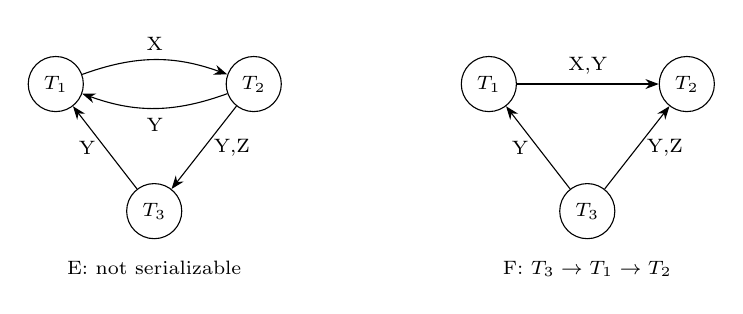
\begin{tikzpicture}[>=Stealth,n/.style={draw,circle,inner sep=1pt,minimum size=7mm},every node/.append style={font=\scriptsize}]
\begin{scope}
\node[n] (1) {$T_1$}; \node[n,right=1.8cm of 1] (2) {$T_2$}; \node[n,below=0.9cm of 1,xshift=1.25cm] (3) {$T_3$};
\draw[->] (1) to[bend left=20] node[above]{X} (2);
\draw[->] (2) to[bend left=20] node[below]{Y} (1);
\draw[->] (2) -- node[right]{Y,Z} (3);
\draw[->] (3) -- node[left]{Y} (1);
\node[below=0.15cm of 3] {E: not serializable};
\end{scope}
\begin{scope}[xshift=5.5cm]
\node[n] (1) {$T_1$}; \node[n,right=1.8cm of 1] (2) {$T_2$}; \node[n,below=0.9cm of 1,xshift=1.25cm] (3) {$T_3$};
\draw[->] (1) -- node[above]{X,Y} (2);
\draw[->] (3) -- node[right]{Y,Z} (2);
\draw[->] (3) -- node[left]{Y} (1);
\node[below=0.15cm of 3] {F: $T_3\to T_1\to T_2$};
\end{scope}
\end{tikzpicture}
\end{exbox}

%=====================================================================
\section{View Serializability and Other Equivalences (Slides 73--79)}

\begin{keybox}[View equivalence of $S$ and $S'$]
\begin{enumerate}
  \item Same transactions and same operations.
  \item \textbf{Same reads-from:} if $r_i(X)$ in $S$ reads the value written by $w_j(X)$ (or the initial value), it does the same in $S'$.
  \item \textbf{Same final write:} if $w_k(Y)$ is the last write of $Y$ in $S$, it is also the last in $S'$.
\end{enumerate}
\textbf{View serializable} = view equivalent to some serial schedule. Idea: every read ``sees'' the same view, and the final DB state is the same.
\end{keybox}

\begin{itemize}
  \item Without blind writes, conflict and view serializability are the \textbf{same}.
  \item With blind writes, conflict serializability is \textbf{stricter}: \emph{every conflict-serializable schedule is view serializable, but not vice versa.}
  \item Testing view serializability is NP-hard, so conflict serializability is used in practice.
\end{itemize}

\begin{exbox}[Slide 77 -- view serializable but not conflict serializable]
$T_1: r_1(X); w_1(X)$,\quad $T_2: w_2(X)$,\quad $T_3: w_3(X)$ \;(blind writes in $T_2,T_3$)\\
$S_a: \ri1X;\ \wi2X;\ \wi1X;\ \wi3X;\ c_1;\ c_2;\ c_3$
\begin{itemize}
  \item \textbf{Conflict:} $\ri1X$ before $\wi2X$ gives $T_1\to T_2$; $\wi2X$ before $\wi1X$ gives $T_2\to T_1$ $\Rightarrow$ cycle $\Rightarrow$ \textbf{not} conflict serializable.
  \item \textbf{View:} compare with serial $T_1T_2T_3$: $r_1(X)$ reads the initial value in both, and the final write is $w_3(X)$ in both $\Rightarrow$ \textbf{view serializable}.
\end{itemize}
\end{exbox}

\textbf{Semantic (debit--credit) equivalence:} addition and subtraction \emph{commute}, so some non-conflict-serializable schedules are still correct.\\
$S_h: \ri1X; \wi1X; \ri2Y; \wi2Y; \ri1Y; \wi1Y; \ri2X; \wi2X$ -- not conflict serializable ($T_1\to T_2$ on $X$, $T_2\to T_1$ on $Y$). But with the semantics
$X{:=}X{-}10;\ Y{:=}Y{-}20;\ Y{:=}Y{+}10;\ X{:=}X{+}20$ (debit, debit, credit, credit) the final result is correct.

%=====================================================================
\section{Transaction Support in SQL (Slides 80--86)}

\begin{itemize}
  \item A single SQL statement is always \textbf{atomic}.
  \item \textbf{No explicit BEGIN} -- a transaction starts implicitly with the first SQL statement.
  \item Every transaction needs an explicit end: \op{COMMIT} or \op{ROLLBACK}.
  \item \op{SET TRANSACTION} sets:
    \begin{itemize}
      \item \textbf{Access mode:} \op{READ ONLY} or \op{READ WRITE}. Default \op{READ WRITE}, unless isolation is \op{READ UNCOMMITTED}, in which case \op{READ ONLY} is assumed.
      \item \textbf{Diagnostic size $n$:} number of conditions held in the diagnostic area (run-time feedback).
      \item \textbf{Isolation level:} \op{READ UNCOMMITTED}, \op{READ COMMITTED}, \op{REPEATABLE READ}, \op{SERIALIZABLE} (default). If all transactions use SERIALIZABLE the execution is serializable; lower levels may violate it.
    \end{itemize}
\end{itemize}

\textbf{Problems allowed by lower isolation levels:}
\begin{itemize}
  \item \textbf{Dirty read} -- reading a value written by a transaction that later fails.
  \item \textbf{Non-repeatable read} -- another transaction changes a value between two reads (seats on a flight).
  \item \textbf{Phantom} -- $T_1$ reads rows matching a condition (EMP with DNO=5); $T_2$ \emph{inserts} a new DNO=5 row; the new row is a \textbf{phantom} record.
\end{itemize}

\begin{center}
\begin{tabular}{@{}lccc@{}}
\toprule
\textbf{Isolation level} & \textbf{Dirty read} & \textbf{Non-repeatable read} & \textbf{Phantom}\\\midrule
READ UNCOMMITTED & Yes & Yes & Yes\\
READ COMMITTED & No & Yes & Yes\\
REPEATABLE READ & No & No & Yes\\
SERIALIZABLE & No & No & No\\
\bottomrule
\end{tabular}\\[2pt]
{\small Table 21.1 -- possible violations per isolation level (``Yes'' = may occur).}
\end{center}

\textbf{Sample SQL transaction:}
\begin{verbatim}
EXEC SQL WHENEVER SQLERROR GOTO UNDO;
EXEC SQL SET TRANSACTION READ WRITE DIAGNOSTICS SIZE 5
                         ISOLATION LEVEL SERIALIZABLE;
EXEC SQL INSERT INTO EMPLOYEE (FNAME, LNAME, SSN, DNO, SALARY)
         VALUES ('Robert', 'Smith', '991004321', 2, 35000);
EXEC SQL UPDATE EMPLOYEE SET SALARY = SALARY * 1.1 WHERE DNO = 2;
EXEC SQL COMMIT;
GOTO THE_END;
UNDO:    EXEC SQL ROLLBACK;
THE_END: ...
\end{verbatim}
If any statement fails, control jumps to \op{UNDO} and the whole transaction (insert + update) is rolled back.

%=====================================================================
\section{Serializability -- Silberschatz View (Slides 87--90)}

\begin{itemize}
  \item \textbf{Assumption:} each transaction preserves consistency $\Rightarrow$ serial execution preserves consistency.
  \item A (possibly concurrent) schedule is \textbf{serializable} if equivalent to a serial schedule. The two forms are \textbf{conflict serializability} and \textbf{view serializability}.
  \item Simplified view: ignore everything except \texttt{read} and \texttt{write}; arbitrary local computation may happen between them.
  \item Instructions $l_i$ and $l_j$ of $T_i,T_j$ \textbf{conflict} iff some item $Q$ is accessed by both and \textbf{at least one writes $Q$}: read/read no; read/write, write/read, write/write yes.
  \item A conflict forces a (logical) temporal order. \textbf{Consecutive non-conflicting instructions can be swapped} without changing the result.
\end{itemize}

\begin{keybox}[Conflict serializability]
If $S$ can be transformed into $S'$ by a series of \textbf{swaps of non-conflicting instructions}, then $S$ and $S'$ are \textbf{conflict equivalent}. $S$ is \textbf{conflict serializable} if it is conflict equivalent to a serial schedule.
\end{keybox}

\begin{exbox}[Swapping example -- Schedule 3 becomes Schedule 1]
\small
Schedule 3 (reads/writes only): $\;r_1(A)\;w_1(A)\;r_2(A)\;w_2(A)\;r_1(B)\;w_1(B)\;r_2(B)\;w_2(B)$
\begin{enumerate}
  \item $r_1(B)$ and $w_2(A)$ touch different items, so swap them; then swap $r_1(B)$ with $r_2(A)$.
  \item Likewise move $w_1(B)$ before $w_2(A)$ and $r_2(A)$.
  \item Result: $r_1(A)\,w_1(A)\,r_1(B)\,w_1(B)\;r_2(A)\,w_2(A)\,r_2(B)\,w_2(B)$ = serial $T_1T_2$ (Schedule 1).
\end{enumerate}
So Schedule 3 is \textbf{conflict serializable}. Schedule 4 is not: $r_1(A)$ before $w_2(A)$ ($T_1\to T_2$) and $r_2(A)$ before $w_1(A)$ ($T_2\to T_1$) form a cycle.
\end{exbox}

%=====================================================================
\section{One-Page Revision}

\begin{tabularx}{\linewidth}{@{}p{3.6cm} X@{}}
\toprule
Transaction & Logical unit of DB work; ops read/write; ends in commit or abort.\\
ACID & Atomicity (all/none), Consistency (valid$\to$valid), Isolation (as if serial), Durability (survives failure).\\
States & Active $\to$ Partially committed $\to$ Committed; Active/Partially committed $\to$ Failed $\to$ Aborted (restart/kill).\\
Concurrency problems & Lost update, dirty read, incorrect summary, unrepeatable read (+ phantom).\\
Failure causes & Crash, transaction error, exception, CC abort, disk failure, catastrophe.\\
Recovery ops & undo (one write), redo (committed write).\\
\#schedules & $(\sum m_i)!\,/\prod m_i!$.\\
Recoverability & Recoverable $\supseteq$ Cascadeless $\supseteq$ Strict; non-recoverable not allowed.\\
Conflict & Same item, different transactions, at least one write.\\
Conflict-serializable test & Precedence graph; acyclic $\Leftrightarrow$ serializable; topological order = serial order.\\
View serializable & Same reads-from + same final writes; conflict-ser. $\subset$ view-ser. (differ only with blind writes).\\
SQL & Implicit begin; COMMIT/ROLLBACK; SET TRANSACTION access mode, diagnostics size, isolation level (default SERIALIZABLE).\\
Isolation table & RU: all 3 anomalies; RC: no dirty read; RR: only phantoms; SER: none.\\
\bottomrule
\end{tabularx}

\end{document}
